\documentclass[aspectratio=169]{beamer}
\usetheme{Madrid}
\usecolortheme{default}

\usepackage{booktabs}
\usepackage{graphicx}
\usepackage{array}

\title[Pythia-160M Alignment Trajectory]{Pythia-160M Repeat-Match Alignment Trajectory}
\subtitle{Cross-seed causal transfer by raw-score alignment versus same head index}
\author{Branch specialization research project}
\date{2026-05-22}

\begin{document}

\begin{frame}
  \titlepage
  \vspace{-0.5em}
  \small
  Checkpoint reason: this is the first Pythia-160M training-trajectory test of
  whether a causal head role transfers across seeds by raw index or by learned
  raw-score alignment.
\end{frame}

\begin{frame}{Question}
  The 14M trajectory showed that repeat-match attention specialization can
  appear before strong causal head importance.

  \vspace{0.8em}
  The stronger 160M question is:

  \vspace{0.5em}
  \begin{center}
  \textit{when the role becomes causal, is it in the same head slot across
  seeds, or in an aligned but relabeled slot?}
  \end{center}

  \vspace{0.8em}
  This separates strong universality from weak, relabeled role universality.
\end{frame}

\begin{frame}{Setup}
  \begin{itemize}
    \item Models: \texttt{EleutherAI/pythia-160m-seed1}, seed2, seed3
    \item Revisions: step0, 1000, 4000, 16000, 64000, 143000
    \item Probe: repeated-token sequences \texttt{[x1,...,x32,x1,...,x32]}
    \item Selected heads: top repeat-match head in layers 0 and 1
    \item Alignment: checkpoint-specific Hungarian matching on raw attention
    scores from four fixed natural probe texts
    \item Causal test: zero selected head outputs, then measure second-half
    continuation loss
  \end{itemize}
\end{frame}

\begin{frame}{Metric Glossary}
  \begin{description}
    \item[Probe specialization] Normalized repeat-match attention score of the
    selected heads. It measures an attention pattern, not causality.
    \item[Own top minus random] Own selected-head loss delta minus random
    same-layer controls. It asks whether the probed heads matter causally.
    \item[Same-index transfer] Ablate the target seed's heads at the source
    seed's original layer/head indices.
    \item[Aligned transfer] Ablate target heads matched to source heads by
    raw-score Hungarian alignment.
    \item[Aligned minus same] Paired advantage of aligned transfer over
    same-index transfer.
  \end{description}
\end{frame}

\begin{frame}{Trajectory}
  \begin{center}
    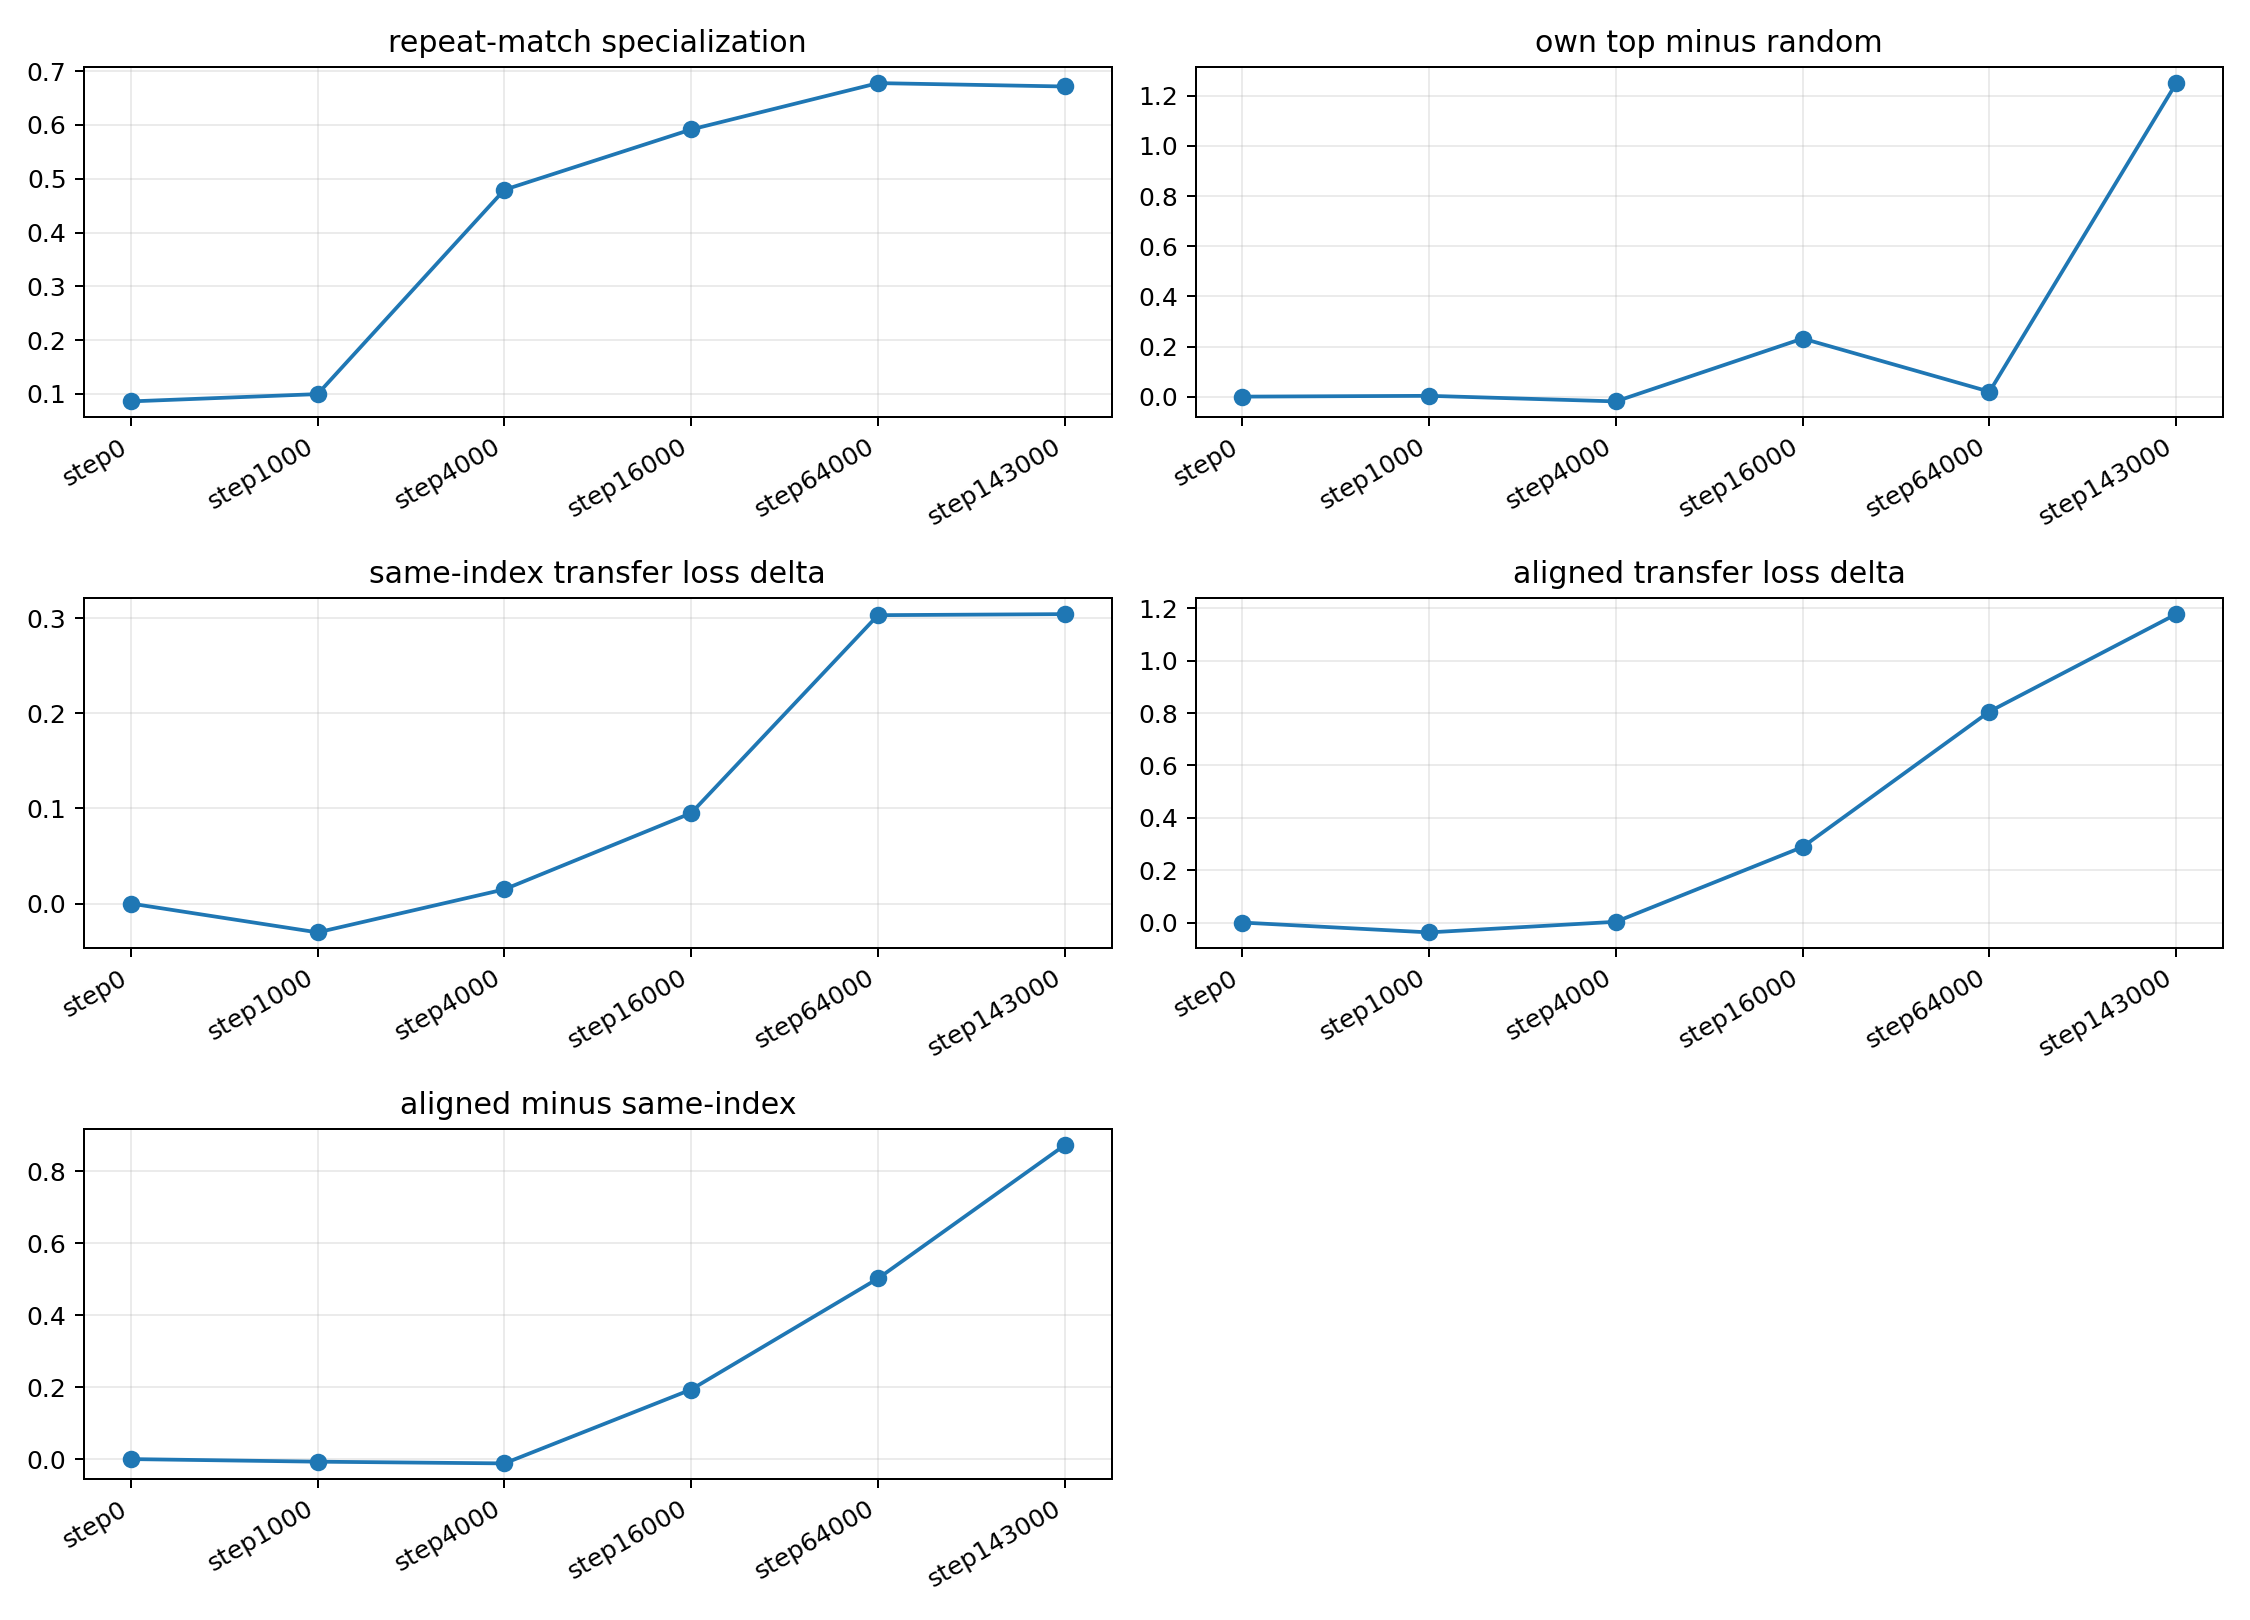
\includegraphics[height=0.70\textheight,keepaspectratio]{figures/repeat_match_alignment_trajectory.png}
  \end{center}

  \small
  Probe specialization rises by step4000, but aligned causal transfer separates
  from same-index transfer mainly from step16000 onward.
\end{frame}

\begin{frame}{Aggregate Results}
  \scriptsize
  \begin{center}
  \begin{tabular}{lrrrrr}
    \toprule
    Revision & Probe spec. & Own top $-$ rand. & Same-index & Aligned & Aligned $-$ same \\
    \midrule
    step0 & 0.0859 & 0.0011 & -0.0000 & 0.0005 & 0.0005 \\
    step1000 & 0.0995 & 0.0042 & -0.0304 & -0.0371 & -0.0067 \\
    step4000 & 0.4794 & -0.0180 & 0.0149 & 0.0034 & -0.0114 \\
    step16000 & 0.5916 & 0.2324 & 0.0952 & 0.2890 & 0.1939 \\
    step64000 & 0.6778 & 0.0206 & 0.3034 & 0.8057 & 0.5023 \\
    step143000 & 0.6715 & 1.2500 & 0.3046 & 1.1774 & 0.8728 \\
    \bottomrule
  \end{tabular}
  \end{center}

  \vspace{0.6em}
  \small
  Means over seeds 1-3. Transfer means use six ordered source-target seed pairs
  per checkpoint.
\end{frame}

\begin{frame}{Paired Transfer Test}
  \small
  \begin{center}
  \begin{tabular}{lrrr}
    \toprule
    Revision & Pairs & Aligned better & Aligned $-$ same mean \\
    \midrule
    step0 & 6 & 4 & 0.0005 \\
    step1000 & 6 & 2 & -0.0067 \\
    step4000 & 6 & 4 & -0.0114 \\
    step16000 & 6 & 5 & 0.1939 \\
    step64000 & 6 & 5 & 0.5023 \\
    step143000 & 6 & 6 & 0.8728 \\
    \bottomrule
  \end{tabular}
  \end{center}

  \vspace{0.8em}
  By the final checkpoint, raw-score alignment beats same-index transfer in all
  six ordered seed pairs.
\end{frame}

\begin{frame}{Interpretation}
  \textbf{Supported}
  \begin{itemize}
    \item Probe specialization appears early: selected-head specialization is
    already 0.4794 by step4000.
    \item Causal importance appears later: own top minus random reaches 0.2324
    at step16000 and 1.2500 at step143000.
    \item Cross-seed causal role identity is mostly relabeled: final aligned
    transfer is 1.1774 versus 0.3046 for same-index transfer.
  \end{itemize}

  \vspace{0.6em}
  \textbf{Not shown}
  \begin{itemize}
    \item This does not prove functional modularity in ordinary Pythia heads.
    \item It validates alignment as a causal role-transfer metric for this
    repeated-token behavior.
  \end{itemize}
\end{frame}

\begin{frame}{Caveats}
  \begin{itemize}
    \item Three seeds only, not the full nine-seed Pythia suite.
    \item Layers 0 and 1 only.
    \item Synthetic repeated-token task.
    \item Alignment uses four natural probe texts; this should be expanded.
    \item Head-output ablation, not full path patching.
    \item Random controls are noisy at step64000, so aligned-vs-same transfer is
    the cleaner cross-seed readout there.
  \end{itemize}
\end{frame}

\begin{frame}{Project-Level Update}
  The Phase 1 story is now stronger:

  \begin{enumerate}
    \item Same head index is a weak carrier of the repeat-match role across
    seeds.
    \item Raw-score alignment reveals the transferable causal role after
    training has progressed far enough.
    \item Probe-defined specialization and causal transfer have different
    developmental timelines.
  \end{enumerate}

  \vspace{0.8em}
  The paper framing should distinguish role existence, causal importance, and
  alignment-based cross-seed identity.
\end{frame}

\begin{frame}{Decision And Next Step}
  \textbf{Decision.} Keep raw-score alignment plus causal transfer as the main
  Phase 1 test of weak universality.

  \vspace{0.8em}
  \textbf{Next step.}
  Scale the 160M result before making paper-level claims:

  \begin{itemize}
    \item run seeds 1-9 at step4000, step16000, and step143000;
    \item expand the alignment probe corpus;
    \item keep same-index transfer as the negative baseline;
    \item optionally add path patching after the ablation result survives.
  \end{itemize}
\end{frame}

\begin{frame}{Provenance}
  \small
  \textbf{Source}
  \begin{itemize}
    \item \texttt{scripts/pythia\_repeat\_match\_alignment\_trajectory.py}
    \item \texttt{scripts/analyze\_pythia\_alignment\_trajectory.py}
    \item \texttt{doc/phase1\_pythia160m\_repeat\_match\_alignment\_trajectory.md}
  \end{itemize}

  \vspace{0.4em}
  \textbf{Copied data}
  \begin{itemize}
    \item \texttt{data/revision\_summary.csv}
    \item \texttt{data/condition\_summary.csv}
    \item \texttt{data/transfer\_pair\_summary.csv}
    \item \texttt{figures/repeat\_match\_alignment\_trajectory.png}
  \end{itemize}

  \vspace{0.4em}
  \textbf{Run command}
  \begin{itemize}
    \item \texttt{python3 -u scripts/pythia\_repeat\_match\_alignment\_trajectory.py --model-size 160m --seeds 1 2 3 ...}
  \end{itemize}
\end{frame}

\end{document}
